\section{Experiments and results}\label{chapter4}




\subsection{Dataset}
We illustrate our two \textsc{nmf} algorithms on two real-world face image datasets: \texttt{ORL} and \texttt{CroppedYaleB} (\citet{belhumeur1997eigenfaces}).
Both \texttt{ORL} and \texttt{CroppedYale} datasets contain multiple images of distinct subjects with various facial expression, lighting condition, and facial details.
Images in ORL are cropped and resized to $92 \times 112$ pixels. We further rescale it to $30 \times 37$ pixels. Similarly, we reduce the size of images in \texttt{CroppedYale} to $42 \times 48$ pixels.
For each dataset, we flatten the image matrix into a vector and append them together to get a matrix $V$ with shape $d\times n$ where integer~$d$ is the number of pixels in one image and integer~$n$ is the number of images. In each epoch, we use 90\% of data.

\subsection{Experiment Setup}
We apply two algorithms (\textsc{nmf} and \textsc{klnmf}) with four categories of noises (no noise, Gaussian noise, Poisson noise and Salt \& Pepper noise), which results in eight combinations in each epoch. In each epoch, we randomly select 90\% of samples to train NMF algorithms and evaluate three metrics on reconstructed images. The training will terminate when the error reaches the minimum error, or the maximum iteration is reached. The minimum error and maximum iteration are hyperparameters which we learn from iterative experiments. Our code saves the learning errors versus the number of iterations so that we could draw the plot and observe the convergence of the learning process. We increase the number of epochs and calculate the average metrics and confidence intervals.

\subsubsection{multiprocessing speed up hyperparameter tuning}
\subsubsection{Hardware and software}

\subsubsection{Early stopping decides maximum number of iterations}

\subsection{Experiments Results}
\subsubsection{Optimal hyperparameters}

Table of results and hyperparameters with optimal and suboptimal coefficients.

\begin{figure}
	\centering
	%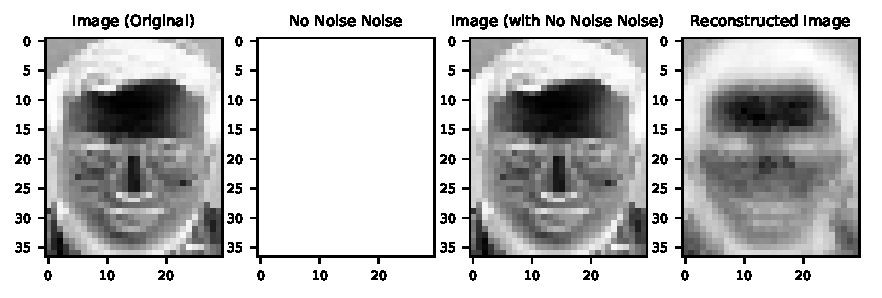
\includegraphics[scale=.9]{Result_Multiplication_KL_Divergence_No_Noise_Comparison}
\caption{Put accuracy vs iteration here with the best possible hyperparameter, and parameters without each of normalisation, dropout, momentum}\label{noisesklnmff}
\end{figure}


\begin{table}
\caption{Results and parameters of the best four setups.}
{\footnotesize
% \label{tab:ci}\begin{tabular}{l|lll}
%  \hline
% \texttt{ORL} dataset & \textsc{rre} & \textsc{acc} & \textsc{nmi}\tabularnewline
%  \hline
% \textsc{nmf} no noise & 0.1583 (0.1581, 0.1584) & 0.7364 (0.731, 0.742) & 0.8536 (0.8506, 0.8567)\tabularnewline
% \hline
% \end{tabular}}
\centering
\begin{tabular}{@{}llllll@{}}
\toprule
Experiment                & Test 1  & Test 2           & Test 3           & Test 4  & Test 5  \\ \midrule
Runtime(mins)             & 2.3     & 2.7              & 3.6              & 17.2    & 10.8    \\
Accurarcy                 & 89.9\%  & 89.7\%           & 89.8\%           & 90.0\%  & 89.3\%  \\
Initialisation            & Xavier  & Uniform$(-1,1)$ & Uniform$(-1,1)$ & Xavier  & Xavier  \\
Batch size                & 1500    & 1500             & 1500             & 1500    & 1500    \\
Hidden layer nodes        & 160     & 150              & 150              & 900     & 160     \\
Activation function       & $\tanh$ & $\tanh$          & $\tanh$          & $\tanh$ & sigmoid \\
Weight decay rate         & 0.0007  & 0.0007           & 0.0007           & 0.007   & 0.007   \\
Momentum rate             & 0.9     & 0.9              & 0.92             & 0.9     & 0.9     \\
Dropout rate              & 0.95    & 1.0              & 1.0              & 0.5     & 0.95    \\
Learning rate             & 0.11    & 0.05             & 0.05             & 0.11    & 0.11    \\
Early stopping iterations & 44      & 54               & 66               & 158     & 282     \\ \bottomrule
\end{tabular}
%\csvautobooktabular{resource/table1.csv}
}
\end{table}

\begin{table}
\caption{Results and parameters of different setups for 89.87 results.}
{\footnotesize \centering
\begin{tabular}{@{}lrrrrr@{}}
\toprule
Experiment                & Test 1  & Mini-Batch & Weight decay & Momentum & Drop out 50\% \\ \midrule
Runtime(minutes)          & 2.3     & 0.5        & 8.6          & 0.8      & 7.6           \\
Accurarcy                 & 89.9\%  & 85.5\%     & 89.4\%       & 88.6\%   & 87.5\%        \\
Initialisation            & Xavier  & Xavier     & Xavier       & Xavier   & Xavier        \\
Batch size                & 1500    & 1500       & 1500         & 1500     & 60000         \\
Hidden layer nodes        & 160     & 160        & 160          & 160      & 160           \\
Activation function       & $\tanh$ & $\tanh$    & $\tanh$      & $\tanh$  & $\tanh$       \\
Weight decay rate         & 0.0007  & 0.0007     & 0.0007       & 0        & 0.007         \\
Momentum rate             & 0.9     & 0.9        & 0            & 0.9      & 0.9           \\
Dropout rate              & 0.95    & 0.5        & 0.95         & 0.95     & 0.95          \\
Learning rate             & 0.11    & 0.11       & 0.11         & 0.11     & 0.11          \\
Early stopping iterations & 44      & 9          & 198          & 16       & 177           \\ \bottomrule
\end{tabular}
}
\end{table}

\begin{figure}
    \center{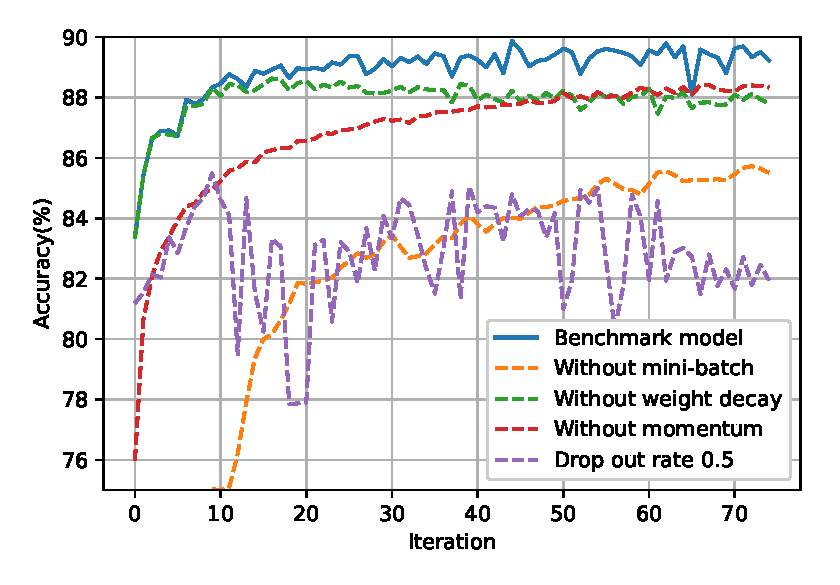
\includegraphics
    {resource/acc.eps}}
    \caption{\label{fig:my-label}Results and parameters of different setups for 89.87 results.}
\end{figure}

\subsection{Experiments Results}
\subsubsection{Vectorisation dramatically improves the speed of training}
\subsubsection{Batch normalisation significantly improves the accuracy}
\subsubsection{Weight decaying prevents overfitting}
\subsubsection{dropout does not help here}
